\section{Implementierung}

Im Folgendem wird auf die Implementierungsdetails der einzelnen Komponenten eingegangen. Hierbei wird der grundlegende Aufbau der Komponenten erklärt.
Zudem wird auf einige Optimierungen und Designentscheidungen eingegangen.


\subsection{Model}

Um Multilayer Graphen in Graph Engine abzubilden wird pro Knoten und Layer eine Zelle erstellt. Die Zellen speichern hierbei ihre ID, ihren Layer, eine Liste der ausgehenden Kanten und die Daten die für die Algorithmen notwendig sind.
Die Kanten müssen dabei speichern, auf welche ID in welchem Layer sie zeigen.

\begin{lstlisting}[language=c,label={lst:tslModel}, caption={TSl Definition von Multilayer Knoten und Kanten.}]
struct Edge {
  long StartId;
  int StartLayer;
  long DestinationId;
  int DestinationLayer;
  float Weight;
}

// We create a cell for each layer a node is on
cell struct Node {
  long Id;
  int Layer;
  PageRankData PageRankData;
  HITSData HITSData;
  DegreeData DegreeData;
  List<Edge> Edges;
}
\end{lstlisting}

Die Proxy wird mit allen unterstützten Protokollen definiert. 

Die Proxy muss von den Servern benachrichtigt werden können, wenn diese asynchrone Aufgaben erfüllt haben. Dabei kann auch ein Ergebnis zurückgegeben werden.
Dafür wird ein \verb|PhaseFinished| Protokoll erstellt. Die Server nutzen das Protokoll, um der Proxy eine \verb|PhaseFinishedMessage| zu senden.

Diese Nachricht enthält die Phase, die beendet wurde und eine Liste an Strings, welche das Ergebnis der jeweiligen Phase darstellt. Es wird hier aus zwei Gründen eine Liste an Strings verwendet. Zum einem gibt es Algorithmen, die ein Ergebnis pro Layer des Graphen zurück gegeben wollen.
Dabei stellt jedes Element der Liste einen Layer des Graphen dar. Zum anderen werden Strings verwendet, da die Ergebnisse verschiedenen Datentypen haben können, welche allerdings alle in einem String dargestellt werden können. So gibt ein Algorithmus, der Knoten zählt nur Integer Werte zurück, wohingegen ein Algorithmus der PageRank Werte zurückgibt Double werte benutzt.
Die Phasen werden in einer separaten TSL Datei verwaltet und als Enum abgespeichert.

Um von der Proxy Ergebnisse zurück an den Client geben zu können, gibt es das Konstrukt \verb|AlgorithmResult|. Dieses beinhaltet ein Ergebnis und die Laufzeit des Algorithmus.


\begin{lstlisting}[language=c, caption={Definition für die Proxy Protokolle.}]

struct AlgorithmResult {
  string Name;
  DateTime StartTime;
  DateTime EndTime;
  List<List<string>> ResultTable;
}

struct StandardAlgorithmMessage {
  AlgorithmOptions AlgorithmOptions;
  OutputOptions OutputOptions;
}

struct PhaseFinishedMessage {
  List<string> Result;
  Phases Phase;
}

protocol PhaseFinished {
  Type: Asyn;
  Request: PhaseFinishedMessage;
  Response: void;
}

proxy MultiLayerProxy {
  // Base Protocols
  protocol PhaseFinished;
  // Data Load Protocols
  protocol LoadGraphProxy;
  ...
  // EgoNetwork
  protocol EgoNetworkProxy
}
\end{lstlisting}


\begin{lstlisting}[language=c, caption={Definition der einzelnen Phasen.}]
// This is a list of all the phases for the different algorithms
// These will be used in the proxies PhaseFinished protocol to identify
// which phase has been finished.
enum Phases {
  // DataLoad Phases
  DataLoad = 0,
  // Stats Phases
  NodeCount = 1,
  EdgeCount = 2,
  ...
  // EgoNetwork
  EgoNetwork = 17
}
\end{lstlisting}


Die einzelnen Algorithmen definieren ihre benötigten Protokolle und Nachrichten in eigenen Dateien. Diese sind jeweils auf den jeweiligen Algorithmus zugeschnitten.
Die Server Definition zieht alle diese Protokolle zusammen, sodass die entsprechenden abstrakten Methoden in der Serverklasse generiert werden.

\subsection{Lib}


Die geteilte Bibliothek stellt eine statische Klasse \verb|Graph| zur Verfügung, die von den anderen Komponenten genutzt wird. Die Klasse ermöglicht es mit dem in Graph Engine gespeicherten Graph zu interagieren, ohne die Implementierungsdetails zu kennen. So kann auf Knoten zugegriffen werden, ohne zu wissen, wie ID und Layer in eine Graph Engine ZellenID übersetzt werden. 
Dazu kommen Funktionen, um Knoten zu erstellen und diese zu verändern.

\subsubsection{Ausgabe}

Die Bibliothenk stellt die Funktionalität zur Ausgabe von Ergebnissen zur Verfügung. Die verschiedenen Arten Ergebnisse auszugeben implementieren alle
das Interface \verb|IOutputWriter|, welches die Funktion \verb|void WriteOutput(AlgorithmResult algorithmResult)| hat. Es gibt drei verschiedene Ausgabearten:

\begin{itemize}
  \item \verb|None|, gibt nichts aus
  \item \verb|Console|, gibt das Ergebnis in der Konsole aus
  \item \verb|CSV|, gibt das Ergebnis in einer .csv Datei aus
\end{itemize}


\subsection{Client}

Der Client kann über die Kommandozeile gestartet und bedient werden. Mit dem Argument 'interactive' wird eine interaktive Sitzung gestartet,
in der der Nutzer Befehle eingeben kann, die die Proxy dann ausführt. Im 'batch' Modus wird zudem eine Datei mitgegeben, die Anweisungen erhält.

Der Client verwaltet eine Liste an ausführbaren Kommandos, die vom Nutzer abgerufen werden können. Dazu speichert er die aktuellen Einstellungen zur Ausführung von Funktionen und Ausgabe der Ergebnisse. Eine Übersicht über die Struktur ist in Abbildung \ref{clientClass} gezeigt.



\subsubsection{Kommandos}

Die einzelnen Funktionen des Clients sind in Kommandos aufgeteilt.
Diese implementieren alle das Interface \verb|ICommand|. Der Client verwaltet ein Dictionary mit allen \verb|ICommands| die er kennt.
Das Interface bietet Zugang zu Informationen über das Kommando, wie z.B. das Keyword, um es aufzurufen oder welche Argumente das Kommando benötigt.
Dazu gibt es drei Interface Funktionen:

\begin{itemize}
  \item \verb|VerifyArguments(string[] arguments)|, prüft ob die Liste der Argumente die der Nutzer dem Kommando gegeben hat legitime Argumente für das Kommando sind.
  \item \verb|ApplyArguments(string[] arguments)|, wendet die Argumente auf das Kommando an sodass es wenn es danach ausgeführt wird die Werte benutzt.
  \item \verb|Run()|, führt das jeweilige Kommando aus.
\end{itemize}

Da die Methoden, die nur Informationen zurückgegeben, sowie das Verifizieren der Argumente für alle Kommandos gleich funktioniert, gibt es eine abstrakte Klasse
\verb|Command|, welche diese bereits implementiert. Die Kommandos erben von dieser Klasse und müssen nur noch \verb|ApplyArguments(string[] arguments)| und \verb|Run()| selbst implementieren.
Die Kommandos füllen die Informationen über sich selbst jeweils in ihrem Konstruktor aus. Diese sind:

\begin{itemize}
  \item \verb|Name|, der Name des Kommandos
  \item \verb|Keyword|, das Keyword um es aufzurufen
  \item \verb|Description|, eine kurze Beschreibung was das Kommando macht
  \item \verb|Arguments|, eine Liste welche die festhält welche Datentypen die Argumente haben
  \item \verb|ArgumentsDescription|, eine Beschreibung für die einzelnen Argumente
\end{itemize}

Die Verifizierung der Argumente findet in zwei Schritten statt. Zuerst wird die Anzahl der gegebenen Argumente mit der Anzahl der Elemente von 'Arguments' verglichen.
Im zweiten Schritt wird für jeden Eintrag in \verb|Arguments| geprüft, ob das gegebene Argument dem jeweiligen Typ entspricht.


\begin{figure}
  \centering
  \begin{subfigure}[b]{1.0\textwidth}
    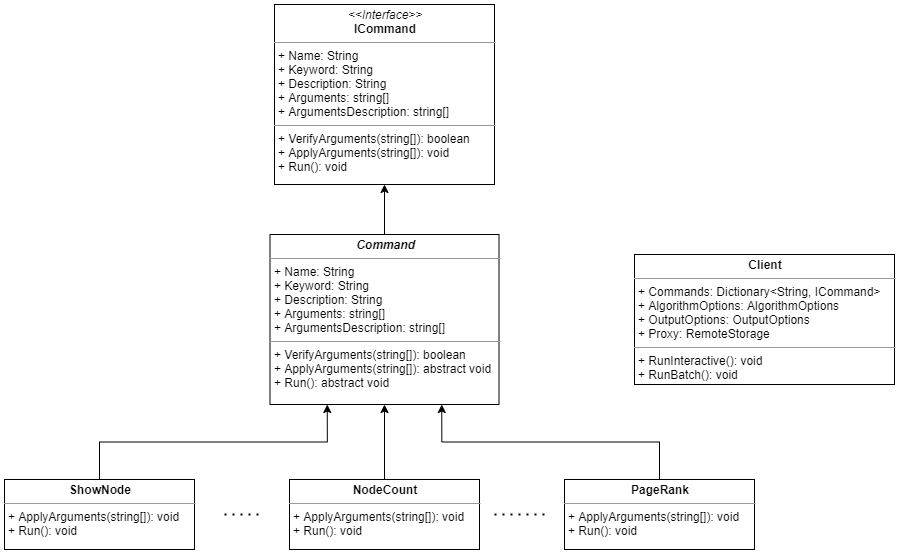
\includegraphics[width=1.0\linewidth]{img/client_class.png}
  \end{subfigure}
  \caption{Klassendiagramm für die Client-Anwendung}
  \label{clientClass}
\end{figure}


\subsubsection{Interaktiver Modus}

Der Batch Modus wird mit dem Argument 'interactive' gestartet. Sobald der Client die Verbindung zum Graph Engine Cluster aufgebaut hat, kann der Nutzer Kommandos eingeben.


\begin{lstlisting}[language=bash]
  $ dotnet run interactive
\end{lstlisting}


\subsubsection{Batch Modus}
 Der Batch Modus wird mit dem Argument 'batch' gestartet. Es muss zudem ein weiteres Argument gegeben werden, welches der Pfad zu der batch Datei ist.

 Diese Datei ist eine normale Textdatei, die pro Zeile ein Kommando enthält. Der Client arbeitet die Datei Zeile für Zeile ab und führt die Kommandos aus.
 Die Verarbeitung verhält sich genau so, als hätte ein Nutzer das Kommando im interaktiven Modus eingegeben. Wird das Ende der Datei erreicht, wird das Client Programm beendet.

\begin{lstlisting}[language=bash]
  $ dotnet run batch path\to\batch\file 
\end{lstlisting}


\subsection{Proxy}



Die in den TSL Dateien definierte Proxy \verb|MultiLayerProxy| wird vom TSL Compiler in eine abstrakte Klasse \verb|MultiLayerProxyBase| mit abstrakten Request Handlern kompiliert. Diese wird hier von 'MultiLayerProxyImpl' implementiert.

Da die \verb|MultiLayerProxyImpl| alle Requests für alle Protokolle handhaben muss, wird sie über mehrere Dateien als partielle Klasse implementiert. Dies vermag die sonst sehr groß werdende Klasse in kleine Teile aufzuteilen, sodass eine Datei jeweils nur für einen Algorithmus verantwortlich ist.
Die Abbildung \ref{proxyClass} gibt eine Übersicht über den Aufbau der Proxy-Anwendung.


\begin{figure}
  \centering
  \begin{subfigure}[b]{1.0\textwidth}
    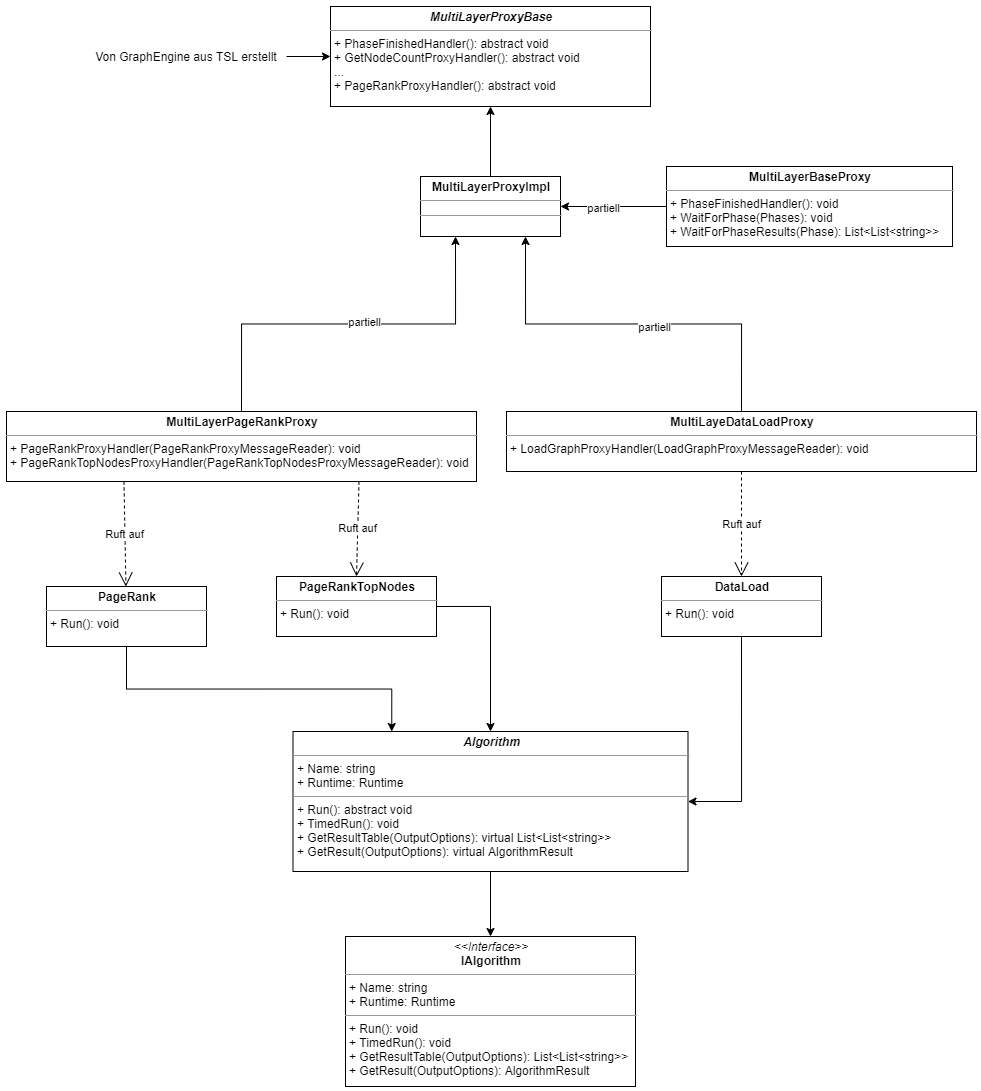
\includegraphics[width=1.0\linewidth]{img/Klassendiagramm-Proxy.png}
  \end{subfigure}
  \caption{Klassendiagramm für die Proxy-Anwendung}
  \label{proxyClass}
\end{figure}


\subsubsection{BaseProxy}

In 'MultiLayerBaseProxy.cs' wird die grundlegende Funktionalität der Proxy definiert, die nicht zu einem einzelnem Algorithmus gehört. Dies ist zum einen die Möglichkeit Algorithmen zu starten und deren Ergebnisse auszugeben, zum anderem wird hier die Möglichkeit geboten auf Antworten der einzelnen Server, sobald diese eine Phase beendet haben, zu warten.
Hat ein Server eine Phase beendet, sendet er an die Proxy einen \verb|PhaseFinished| Request, der die Phase enthält, die er beendet hat und wenn nötig sein lokales Ergebnis. Die \verb|MultiLayerBaseProxy| handhabt diesen Request und zählt wieviele Server eine jeweilige Phase schon beendet haben und sammelt deren Ergebnisse. Hierfür werden drei Elemente verwendet:

\begin{itemize}
  \item \verb|Dictionary<Phases, int> phaseFinishedCount|, um zu zählen ,wieviele Server bereits eine bestimmte Phase abgeschlossen haben.
  \item \verb|List<List<string>> phaseResults|, um die Ergebnisse der einzelnen Server zu aggregieren
  \item \verb|object phaseFinishedCountLock|, dient als Lock, um die Operationen an den anderen beiden Variablen zu schützen
\end{itemize}

Es wird solange gewartet, bis die Anzahl an Servern, die eine Phase als beendet gemeldet haben, der Anzahl aller Server entspricht.

\begin{lstlisting}[language=c, caption={Implementierung des Mechanismus, um auf Phasen zu warten.}]
public override void PhaseFinishedHandler(PhaseFinishedMessageReader request) {
  // Lock the phaseFinishedCount to avoid lost updates.
  lock (phaseFinishedCountLock) {
    phaseResults.Add(request.Result);
    phaseFinishedCount[request.Phase]++;
  }
}

private void WaitForPhaseAnswers(Phases phase) {
  SpinWait wait = new SpinWait();

  while (phaseFinishedCount[phase] != Global.ServerCount) {
    wait.SpinOnce();
  }

  lock (phaseFinishedCountLock) {
    phaseFinishedCount[phase] = 0;
  }
}
\end{lstlisting}

Die Proxy bietet den einzelnen Algorithmen damit die Möglichkeit, auf Ergebnisse zu warten. Außerdem gibt es mehrere Methoden, die es erlauben, die Ergebnisse direkt im gewünschten Datentyp zu erhalten.

\subsubsection{Algorithmen}

Um die Ausführung, Perfomance Messung und Ausgabe von Ergebnissen einheitlich zu halten, gibt es das Interface \verb|IAlgorithm|, welches die Grundfunktionen der Algorithmen definiert(siehe Abbildung \ref{proxyClass}).
Es besitzt vier Methoden:

\begin{itemize}
  \item \verb|Run()|, führt den Algorithmus aus
  \item \verb|TimedRun()|, führt den Algorithmus aus und misst die Laufzeit
  \item \verb|List<List<string>> GetResultTable(OutputOptions outputOptions)|, gibt das Ergebnis in Tabellenform zurück
  \item \verb|AlgorithmResult GetResult(OutputOptions outputOptions)|, gibt das komplette Ergebnis inklusive Laufzeit zurück
\end{itemize}

Das Interface wird von der abstrakten Klasse \verb|Algorithm| implementiert. In dieser Klasse bleibt die \verb|Run()| Methode abstrakt.
Die Klassen für die einzelnen Algorithmen erben von \verb|Algorithm| und implementieren entsprechend ihrer Anforderungen die \verb|Run()| Methode.

Erhält die Proxy eine Anfrage einen bestimmten Algorithmus auszuführen ruft der entsprechende Requesthandler den angefragten Algorithmus auf.



\subsection{Server}

Wie schon bei der Proxy wird der in TSL definierte Server \verb|MultiLayerServer| zu der abstrakten Klasse \verb|MultiLayerServerBase| kompiliert. Diese hat abstrakte Methoden für die Protokollhandler.
Die \verb|MultiLayerServerBase| wird von der Klasse \verb|MultiLayerServerImpl| implementiert, welche auch wieder zur besseren Übersicht in einzelne partielle Klassen aufgeteilt wird. Diese partiellen Teile sind in die jeweiligen Algorithmen und eine Basisklasse \verb|MultiLayerBaseServer| aufgeteilt.
Der \verb|MultiLayerBaseServer| bietet den Algorithmen Methoden, um der Proxy mitzuteilen, dass sie eine Phase beendet haben.
Der Aufbau der Server-Anwendung ist in Abbildung \ref{serverClass} dargestellt.


\begin{figure}
  \centering
  \begin{subfigure}[b]{1.0\textwidth}
    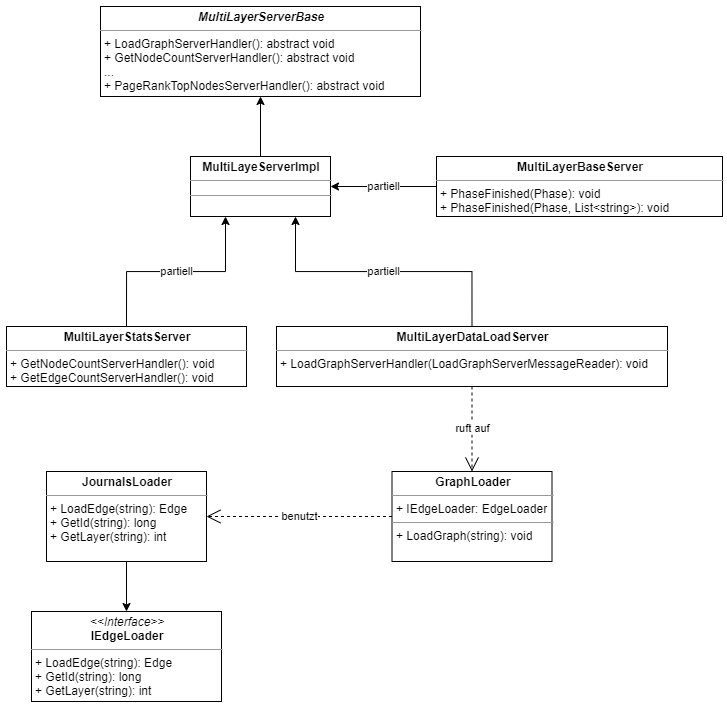
\includegraphics[width=1.0\linewidth]{img/Klassendiagramm-Server.png}
  \end{subfigure}
  \caption{Klassendiagramm für die Server-Anwendung}
  \label{serverClass}
\end{figure}


\subsubsection{Laden}

Das Laden des Graphen findet verteilt über alle vorhandenen Server statt. Die Kanten werden von einer Kantendatei geladen, die je eine Kante pro Zeile speichert. Das genaue Format, wie eine Kante in dieser Kantendatei vorhanden ist, kann verschieden sein. Wichtig ist das jede Kante die Informationen enthält, von welchem Knoten und Layer zu welchem Knoten und Layer sie zeigt.

Jeder Server geht die Kantendatei Zeile für Zeile durch und puffert diese in einer Liste. Die Liste wird solange gefüllt, bis der Knoten wechselt, von dem die Kanten ausgehen. Sobald der Knoten wechselt, wird die gepufferte Liste von Kantenzeilen an einen Threadpool übergeben, der die Kantenzeilen lädt und den Knoten in Graph Engine speichert.

Um mehrere Formate an Kantenzeilen zu unterstützen, gibt es ein Interface \verb|IEdgeLoader|. Dieses stellt drei Methoden zur verfügung die implementiert werden müssen.

\begin{itemize}
  \item \verb|Edge LoadEdge(string line)|, lädt eine Kante aus einer Zeile
  \item \verb|long GetId(string line)|, liest die Knoten ID aus einer Zeile aus
  \item \verb|int GetLayer(string line)|, liest den Layer aus einer Zeile aus
\end{itemize}

Die Methoden \verb|GetId| und \verb|GetLayer| sind nötig, damit während des Pufferns der Zeilen festgestellt werden kann, wann der Ursprungsknoten der Kanten wechselt.
Für alle Formate, die unterstützt werden sollen, muss nun eine Klasse erstellt werden, die das Interface implementiert.


\subsection{Algorithmen}

Für das Multilayer Graph System wurden bereits Algorithmen bzw. Metriken implementiert. In diesem Abschnitt wird grob die Funktionsweise der einzelnen Algorithmen und deren Optimierungen erläutert.


\subsubsection{Knoten- und Kantenanzahl}
Zum bestimmen der Knote- und Kantenanzahl zählt jeder Server die Knoten bzw. deren Kanten für die er verantwortlich ist. Dabei kann bei der Kantenanzahl festgelegt werden, ob Kanten die von einem Layer in einen anderen gehen mitgezählt werden.
Die Knoten und Kanten werden pro Layer gezählt und das Ergebnis an die Proxy gesendet. Diese zählt die Ergebnisse aller Server zusammen und bildet das Endergebnis.
 

\subsubsection{Graph Dichte}

Die Graph Dichte wird berechnet, indem die Proxy einmal die Knoten und Kanten, wie zuvor beschrieben zählt.
Danach wird für jeden Layer die Dichte wie in \ref{dichte} beschrieben berechnet.


\subsubsection{Knotengrad}

Der Knotengrad für jeden Knoten wird in zwei Schritte ermittelt.
Da jeder Knoten seine ausgehenden Kanten speichert kann der Ausgangsgrad einfach bestimmt werden. Jeder Server zählt für seine Knoten die Anzahl der ausgehenden Kanten.

Um den Eingangsgrad zu bestimmten geht jeder Server alle seine Knoten durch. Für jede Kante wird geprüft, ob der Zielknoten auf dem gleichen Server liegt. Ist dies der Fall wird der Eingangsgrad des Knoten direkt um 1 erhöht.
Liegt der Knoten auf einem anderen Server wird diesem eine entsprechende Nachricht zugesandt und dieser erhöht den Eingangsgrad des Knoten.


\subsubsection{PageRank}

Das Berechnen der PageRank Werte ist in mehrere Phasen aufgeteilt, deren Ablauf von der Proxy gesteuert wird.

In einer ersten Phase werden die Werte für alle Knoten auf den gleichen initial Wert gesetzt. Dieser kann vom Client gewählt werden.

Danach beginnt die Update Phase, in der die Werte neu berechnet werden. Hier wird, wie in \ref{pageRank} beschrieben, jeweils der neue Wert für jeden Knoten berechnet.
Dabei geht jeder Server alle seine Knoten und deren Kanten durch. Falls der Zielknoten der Kante auf dem gleichen Server liegt kann der Wert sofort entsprechend geändert werden.
Liegt der Zielknoten auf einem anderen Server wird sich gemerkt, um wieviel der Wert sich ändern muss und dies dem entfernten Server per Nachricht mitgeteilt.


Sind alle Updates abgeschlossen wird die Normalisierung der Werte durchgeführt und bestimmt, wie groß die Gesamtänderung aller PageRank Werte ist.
Liegt die Gesamtänderung unter einem vom Client gewählten $\epsilon$ wird der Algorithmus beendet. Ansonsten wird eine weitere Update Runde durchgeführt.


\subsubsection{HITS}

Zum bestimmen der Hub und Authority Werte läuft der Algorithmus in mehren Phasen ab, die von der Proxy gesteuert werden.

In der ersten Phase werden die Hub und Authority Werte auf einen vom Client festgelegten initial Wert gesetzt.

Danach werden erst die Authority Werte neu berechnet. Dabei wird über jeden Knoten und jede Kante iteriert. Zeigt die Kante auf einen lokalen Knoten kann dessen Authority Werte direkt angepasst werden. Handelt es sich um einen entfernten Knoten auf einem anderen Server
wird diesem eine Nachricht mit der Wertänderung geschickt.

Sind die Authority Werte neu berechnet werden diese in einer weiteren Phase normalisiert. Dabei wird die Gesamtänderung der Authority Werte bestimmt und der Proxy mitgeteilt.

Danach werden die neuen Hub Werte berechnet. Dazu iteriert jeder Server über alle seine Knoten und deren Kanten. Zeigt die Kante auf einen lokalen Knoten wird dessen Authority Wert genutzt, um den Hub Wert des aktuellen Knotens zu aktualisieren.
Handelt es sich um einen entfernten Knoten wird sein Authority Wert von dem anderen Server angefragt. 

Anschließen werde auch die Hub Werte normalisiert und deren Gesamtänderung berechnet. Dieser wird der Proxy zugesandt.

Die Proxy prüft nun, ob die Gesamtänderung der Hub und Authority Werte unter einem vom Client gewählten Schwellwert $\epsilon$ liegt. Ist dies nicht der Fall wird wieder mit dem Update der Authority Werte begonnen.


\subsubsection{Optimierungen}

Algorithmen, wie PageRank oder HITS müssen auf Werte von Knoten, die auf anderen Servern gespeichert sind, zugreifen.
Entweder müssen die entfernten Werte aktualisiert oder gelesen werden. Diese Zugriffe direkt zu machen ist, wie in \ref{datenzugriff} erläutert, nicht sehr schnell und erfordert jedes mal Kommunikation zwischen den Servern.
Da diese Kommunikation jedes mal mit einem gewissen Overhead an Aufwand verbunden ist und für große Graphen mehrere Millionen mal auftritt, muss versucht werden dies zu vermeiden.

Als Lösung für das Problem unterstützt das Multilayer Graph System das verschicken von einer Menge an Schlüssel und Werten Paaren in einer Anfrage. Damit wird der Overhead für die vielen einzelnen Anfragen vermieden.
Die Implementierung von PageRank, HITS und der Berechnung des Knotengrads verwenden diese Lösung, um entfernte Werte anzufragen oder zu aktualisieren.


\subsection{Erweiterbarkeit}

Das System ist um weitere Funktionen erweiterbar. In diesem Abschnitt wird erläutert, welche Schritte notwendig sind, um neue Funktionalität hinzuzufügen.
Dabei muss die gewünschte Funktionalität im Model, Client, Proxy und Server hinzugefügt werden.

Um den Ablauf zu veranschaulichen, wird dies für eine Beispielfunktion erklärt. Diese zählt die Anzahl an Knoten, die eine vom Client bestimmte Anzahl an ausgehenden Kanten besitzt.

\subsubsection{Model}

Im Model muss eine .tsl Datei für den neuen Algorithmus erstellt werden. In dieser werden die Daten und Protokolle die Graph Engine unterstützen muss beschrieben. Im Fall der Beispielfunktion sind zwei Protokolle notwendig.
Eines damit der Client die Anfrage für die Ausführung an die Proxy senden kann und ein weiteres, damit die Proxy die einzelnen Server nach ihrer Anzahl an Knoten mit der gewünschten Menge an Kanten fragen kann.
Dabei müssen bei beiden Protokollen die Anzahl der Kanten mitgegeben werden können.

In der Anfrage an die Proxy sollen zudem die Optionen für die Ausführung von Algorithmen, sowie die Option für die Ausgabe von Ergebnissen dabei sein.

\begin{lstlisting}{language=c}
// Proxy Protocol
struct GetNEdgeNodesProxyMessage {
  AlgorithmOptions AlgorithmOptions;
  OutputOptions OutputOptions;
  int NumberOfEdges;  
}

protocol GetNEdgeNodesProxy {
  Type: Syn;
  Request: GetNEdgeNodesProxyMessage;
  Response: void;
}

// Server Protocol
struct GetNEdgeNodesServerMessage {
  int NumberOfEdges;
}

protocol GetNEdgeNodesServer {
  Type: Syn;
  Request: GetNEdgeNodesServerMessage;
  Response: void;
}
\end{lstlisting}

Diese Protokolle müssen nun in \verb|MultiLayerProxy| und \verb|MultiLayerServer| eingetragen werden, damit die von TSL erzeugte Server/Proxy Basisklasse abstrakte Methoden für diese besitzen.

Damit die Server der Proxy ihre lokalen Ergebnisse zusenden können, muss die 'Phases.tsl' Datei um eine Phase für diesen Algorithmus erweitert werden.

\begin{lstlisting}{language=c}
enum Phases {
  // DataLoad Phases
  DataLoad = 0,
  ...
  NEdgesCount = 18
}
\end{lstlisting}


\subsubsection{Client}

Für den neuen Algorithmus muss im Client ein Kommando hinzugefügt werden, um diesen auszuführen. Das Kommando muss dabei die Anzahl der Kanten als Argument nehmen und das zuvor definierte Protokoll nutzen, um die Anfrage an die Proxy zu senden.

Es wird eine neue Klasse \verb|NEdgesNodeCount| erstellt, welche von der abstrakten Klasse \verb|Command| erbt. Im Konstruktor müssen nun die bereits erwähnten Daten eingegeben werden. Dabei ist wichtig, dass es ein Argument des Typs \verb|int| gibt, welches die Anzahl der gewünschten Kanten darstellt.
Nun müssen die Methoden \verb|ApplyArguments| und \verb|Run| implementiert werden.
In \verb|ApplyArguments| wird das übergebene Argument in einer lokalen Variable gespeichert, sodass es beim Aufruf von \verb|Run| verwendet werden kann.
In \verb|Run| wird die im Model bereits definierte Nachricht erstellt und an die Proxy gesendet.

\begin{lstlisting}{language=c}
using MultiLayerLib;
using MultiLayerLib.MultiLayerProxy;

namespace MultiLayerClient.Commands {

  class NEdgesNodeCount: Command {

    private int NumberOfEdges { get; set; }

    public NEdgesNodeCount (Client client): base (client) {
      Name = "NEdge Node Count";
      Keyword = "nEdgeNodeCount";
      Description = "Counts the number of nodes that have a certain amount of edges.";
      Arguments = new string[] { "int" };
      ArgumentsDescription = new string[] { "NumberOfEdges" };
    }

    public override void ApplyArguments(string[] arguments) {
      NumberOfEdges = int.Parse(arguments[0]);
    }

    public override void Run() {
      using (var msg = new GetNEdgeNodesProxyMessageWriter(Client.AlgorithmOptions, Client.OutputOptions, NumberOfEdges)) {
          MessagePassingExtension.GetNEdgeNodesProxy(Client.Proxy, msg);
      }      
    }
  }
}
\end{lstlisting}


In der \verb|Client| Klasse muss im Konstruktor nun noch das erstellte Kommando registriet werden.

\subsubsection{Proxy}

Für die Proxy müssen zwei Funktionen implementiert werden. Zum einem der Algorithmus der Anfragen an alle Server sendet, um ihre Anzahl an lokalen Knoten mit N Kanten zu senden und diese Ergebnisse aggregiert. Zum anderem muss 
für das in TSL definierte Proxy Protokoll \verb|GetNEdgeNodesProxy| ein entsprechender Handler erstellt werden, der die Anfrage verarbeitet und den Algorithmus startet.

Der Algorithmus muss die abstrakte Klasse \verb|Algorithm| implementieren, insbesondere die abstrakte Methode \verb|Run()| und \verb|AlgorithmResult GetResult(OutputOptions outputOptions)|. In \verb|Run()| wird die im Model erstellte Anfrage an alle Server gesendet, welche auf diese mit ihrer lokalen Anzahl an Knoten mit der gewünschten Kantenanzahl antworten. Die Proxy
wartet bis alle Server Ergebnisse gesendet haben und zählt diese zu einem Gesamtergebnis zusammen.

Die andere Methode dient dazu, die Ergebnisse in einer Tabellenform darzustellen. Dazu wird die Anzahl der Knoten pro Layer vermerkt und jeder Layer als eine Reihe in der Tabelle dargestellt. Bei der ersten Spalte handelt es sich um die ID des Layers, während die zweite die Anzahl der Knoten in diesem Layer darstellt. Es wird eine weitere Zeile mit der Gesamtanzahl der Knoten hinzugefügt.

\begin{lstlisting}{language=c}

public override void Run() {
  foreach(var server in Global.CloudStorage) {
    MessagePassingExtension.GetNEdgeNodesServer(server);
  }

  List<List<long>> phaseResults =  Proxy.WaitForPhaseResultsAsLong(Phases.NEdgesCount);
  long[] nodeCount = new long[phaseResults[0].Count];

  // Sum up the results from all the servers.
  foreach(List<long> result in phaseResults) {
    for (int i = 0; i < result.Count; i++) {
        nodeCount[i] += result[i];
    }
  }
}

public override List<List<string>>  GetResultTable(OutputOptions options) {
  List<List<string>> output = new List<List<string>>();
  long totalNodeCount = 0;

  for (int i = 0; i < nodeCount.Length; i++) {
      List<string> outputRow = ResultHelper.Row("Layer" + (i + 1), nodeCount[i].ToString()); 
      output.Add(outputRow);

      totalNodeCount += nodeCount[i];
  }


  output.Add(ResultHelper.Row("Toal", totalNodeCount.ToString()));

  return output;
}



\end{lstlisting}


Der Request Handler muss Teil der partiellen Klasse \verb|MultiLayerProxyImpl| sein. Dafür kann entweder eine weitere Datei erstellt werden oder eine bereits vorhandene genutzt werden die thematisch zu dem Handler passt.
Da Knotenzählen bereits in \verb|MultiLayerStatsProxy| implementiert ist wird dort auch der Handler für \verb|GetNEdgeNodesProxy| hinzugefügt. Dieser muss die Anfrage erhalten, um den Algorithmus zu starten und dann die Ergebnisse auszugeben.

\begin{lstlisting}{language=c}
using MultiLayerProxy.Algorithms;
using MultiLayerLib;

namespace MultiLayerProxy.Proxy {

  partial class MultiLayerProxyImpl: MultiLayerProxyBase {

    public override void GetNEdgeNodesProxyHandler(GetNEdgeNodesProxyMessageReader request) {
      NodeCount nEdgesnodeCount = new NEdgesnodeCount(this, request.NumberOfEdges);

      RunAlgorithm(nEdgesnodeCount, request.AlgorithmOptions);
      OutputAlgorithmResult(nEdgesnodeCount, request.OutputOptions);
    }
  
    // Rest of the class ommitted
  }
}
\end{lstlisting}



\subsubsection{Server}

Auf der Serverseite müssen zwei Funktionen implementiert werden. Der Request im Model definierte Handler \verb|GetNEdgeNodesServer|, welcher von der Proxy aufgerufen wird. Dieser muss die Anfrage verarbeiten und die Funktion zur Berechnung der Kantenanzahl starten. Das Ergebnis dieser Funktion muss wieder zurück an die Proxy gesendet werden.
Dazu muss natürlich die Funktion implementiert werden, welche die Kantenanzahl zählt.

Der Request Handler passt auch hier thematisch wieder zu der bereits vorhandenen Datei \verb|MultiLayerStatsServer|, der eine parteille Klasse der Server Implementierung ist. So wird der Handler hier hinzugefügt.
Es wird das Parameter \verb|NumberOfEdges| aus der Anfrage gelesen und der Funktion zur Berechnung übergeben. Da die Ergebnisse als String Liste an die Proxy übergeben werden müssen, werden diese zu String konvertiert.


\begin{lstlisting}{language=c}
public override void GetNEdgeNodesServerHandler(GetNEdgeNodesServerMessageReader request) {
  List<long> result = Stats.GetNEdgeNodes(request.NumberOfEdges);

  PhaseFinished(Phases.NEdgesCount, Util.ToStringList(result));
}
\end{lstlisting}

Die Funktion zur Berechnung selbst wird als statische Funktion der bereits vorhandenen Klasse \verb|Stats| realisiert. Gäbe es keine passende Klasse, kann diese natürlich nach Bedarf erstellt werden.
In der Funktion selbst wird über alle lokalen Knoten iteriert und die Anzahl der Knoten mit der gewünschten Kantenanzahl pro Layer gezählt. 

Das Ergebnis wird zurück an die Proxy gesendet.

\begin{lstlisting}{language=c}
public static List<long> GetNEdgeNodeCount(int numberOfEdges) {
  long[] nodeCount = new long[Graph.LayerCount];

  foreach(Node_Accessor node in Graph.NodeAccessor()) {
    // Only count nodes with the correct amount of edges
    if (node.Edges.Count == numberOfEdges) {
      nodeCount[node.Layer - 1]++;
    }
  }

  List<long> result = new List<long>(nodeCount);
  return result;
}
\end{lstlisting}




